\section{\texorpdfstring{$L^p$}{Lp}空间}
\label{sec:nspace-lp-spaces}

上一节的折线列在积分误差下彼此越来越近，极限却是一个阶跃函数，不在连续函数之中。本节允许一般的可测函数，按$p$次幂累计偏差，并把在零测集上改动的函数看作同一个元素。这样得到的$L^p$空间满足范数公理，而且完备。

本节固定测度空间$(X,\mathcal A,\mu)$。可测函数、积分、单调收敛定理与Fatou引理见第~\ref{chap:measure}章和第~\ref{chap:integration}章。函数取值于$\mathbb K$，所有估计都只用到绝对值，实、复两种情形的论证相同。

\paragraph{几乎处处相等的函数}
在$[0,1]$上取Lebesgue测度，令$f\equiv0$，而$g$只在$x=\tfrac12$处取$1$、其余处取$0$。单点集的测度为零，所以$\int_0^1\lvert f-g\rvert\,dx=0$。用积分衡量误差时，这两个函数无法区分；若坚持把它们当作不同的元素，积分就只是半范数，正定性失效。

解决办法是把它们看作同一个元素。对两个可测函数，规定
\begin{equation}
 f\sim_\mu g\quad\Longleftrightarrow\quad \mu(\{x:f(x)\neq g(x)\})=0,
 \label{eq:nspace-ae-equivalence}
\end{equation}
即$f=g$在$\mu$下\term{几乎处处}（almost everywhere）成立。这是等价关系：自反与对称直接成立；若$f\sim_\mu g$且$g\sim_\mu h$，则
\[
 \{f\neq h\}\subseteq\{f\neq g\}\cup\{g\neq h\},
\]
两个零测集之并仍是零测集。与$f$几乎处处相等的可测函数全体记为$[f]$，称为$f$的\term{等价类}（equivalence class），$f$是它的一个代表。

等价类之间的运算借助代表定义：$[f]+[g]=[f+g]$，$c[f]=[cf]$。结果不依赖代表的选择：若$f'\sim_\mu f$、$g'\sim_\mu g$，则
\[
 \{f'+g'\neq f+g\}\subseteq\{f'\neq f\}\cup\{g'\neq g\}
\]
是零测集。所以可测函数的等价类组成线性空间，零元素是几乎处处为零的函数这一整类。

把函数看作向量时，这一步相当于放弃了“读取单个分量”。在Lebesgue测度下每个单点都是零测集，同一类中的代表可以在任意给定点取任意值，“$[f]$在$x_0$处的值”没有意义。若$\mu(\{x_0\})>0$，同一类的代表在$x_0$处必须取同一个值。点值读取何时有意义，是第~\ref{chap:linear-functionals}章和第~\ref{chap:rkhs}章的问题。

\paragraph{\texorpdfstring{$L^p$}{Lp}范数}
有了等价类，就可以用$p$次幂的积分衡量函数的大小。这相当于把向量的$p$范数$(\sum_i\lvert v_i\rvert^p)^{1/p}$中的求和换成积分。

\begin{definition}[$L^p$空间]
\label{def:nspace-lp}
设$1\leq p<\infty$。若可测函数$f$满足$\int_X\lvert f\rvert^p\,d\mu<\infty$，称$f$是$p$次可积的。$p$次可积函数的几乎处处等价类全体记为$L^p(\mu)$，并令
\begin{equation}
 \lVert f\rVert_p=\Bigl(\int_X\lvert f\rvert^p\,d\mu\Bigr)^{1/p}.
 \label{eq:nspace-lp-norm}
\end{equation}
当$X$是欧氏空间的可测子集$\Omega$、$\mu$为Lebesgue测度时，记为$L^p(\Omega)$。
\end{definition}

这里用代表$f$代写等价类$[f]$。定义需要核验三件事。其一，数值不依赖代表：若$f\sim_\mu g$，则$\lvert f\rvert^p$与$\lvert g\rvert^p$几乎处处相等，零测集上的改动不影响积分。其二，正定性：$\int\lvert f\rvert^p\,d\mu=0$当且仅当$\lvert f\rvert^p=0$几乎处处，即$[f]$是零元素，这正是引入等价类要换取的结果。齐次性直接由积分的线性得到。

其三，$L^p(\mu)$对加法封闭。$p\geq1$时函数$t\mapsto t^p$在$[0,\infty)$上凸，所以对$a,b\geq0$有
\[
 \Bigl(\frac{a+b}2\Bigr)^p\leq\frac{a^p+b^p}2,
\]
也就是$(a+b)^p\leq2^{p-1}(a^p+b^p)$。取$a=\lvert f(x)\rvert$、$b=\lvert g(x)\rvert$，由$\lvert f+g\rvert\leq a+b$积分得
\[
 \int_X\lvert f+g\rvert^p\,d\mu\leq2^{p-1}\Bigl(\int_X\lvert f\rvert^p\,d\mu+\int_X\lvert g\rvert^p\,d\mu\Bigr)<\infty.
\]
数乘只把积分乘以常数$\lvert c\rvert^p$，封闭性同样成立，所以$L^p(\mu)$是线性空间。剩下的三角不等式不能由这个粗略估计得到，要用下面的Hölder不等式。

\paragraph{不同的\texorpdfstring{$p$}{p}}
$p$越大，局部的大偏差在总量中所占的比重越大。比较$[0,1]$上的两个误差：$h_1\equiv1$处处偏差为$1$，$h_2=4\cdot\mathbf 1_{[0,1/4]}$只在四分之一的区间上偏差为$4$。按绝对值累计，两者一样大：
\[
 \lVert h_1\rVert_1=1,\qquad \lVert h_2\rVert_1=4\times\frac14=1.
\]
按平方累计，分散的误差仍是$1$，集中的误差翻了一倍：
\[
 \lVert h_1\rVert_2=1,\qquad \lVert h_2\rVert_2=\Bigl(16\times\frac14\Bigr)^{1/2}=2.
\]

一般地，同样的计算给出
\[
 \lVert h_2\rVert_p=\Bigl(4^p\cdot\frac14\Bigr)^{1/p}=4^{1-1/p},
\]
它随$p$增大而增大，趋于最大偏差$4$，见图~\ref{fig:nspace-lp-weight}。选择$p$就是选择怎样为大偏差计价。

\begin{BookInlineFigure}
  \centering
  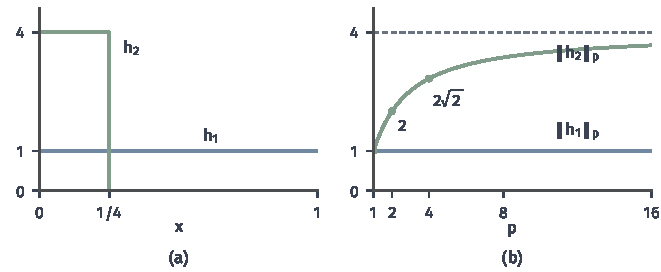
\includegraphics[width=112mm]{figures/04-spaces-measures-and-geometry/03-function-spaces/matplotlib/nspace-lp-weight/figure.pdf}
  \caption{$L^p$范数对大偏差的计价。(a)$[0,1]$上的两个误差：蓝色的$h_1\equiv1$与绿色的$h_2=4\cdot\mathbf 1_{[0,1/4]}$，二者$L^1$范数都是$1$。(b)$\lVert h_1\rVert_p\equiv1$，而$\lVert h_2\rVert_p=4^{1-1/p}$，在$p=1,2,4$处依次为$1,2,2\sqrt2$，虚线是$p\to\infty$时的极限$4$。}
  \label{fig:nspace-lp-weight}
\end{BookInlineFigure}

可积性也随$p$改变。在$(0,1]$上，$x^{-1/2}$属于$L^1$，因为
\[
 \int_0^1x^{-1/2}\,dx=2.
\]
它不属于$L^2$，因为$\int_0^1x^{-1}\,dx=\infty$。$x^{-1/4}$属于$L^2$，平方积分为$2$，但它在$0$附近无界。

\paragraph{数列空间}
取$X=\mathbb N_+$与\term{计数测度}（counting measure），即每个点的测度为$1$。可测函数就是数列$x=(x_k)$，积分就是求和，只有空集零测，等价类就是数列本身。$L^p$成为
\begin{equation}
 \ell^p=\Bigl\{x:\ \sum_{k\geq1}\lvert x_k\rvert^p<\infty\Bigr\},\quad \lVert x\rVert_p=\Bigl(\sum_{k\geq1}\lvert x_k\rvert^p\Bigr)^{1/p}.
 \label{eq:nspace-ellp}
\end{equation}
这是函数作为无限维向量最直接的情形：有限维向量可以看作后面全为零的数列，$\lVert x\rVert_p$就是卷二的坐标$p$范数的延伸。数列$x_k=1/k$属于$\ell^2$，因为$\sum_k1/k^2$收敛；它不属于$\ell^1$，因为调和级数发散。

\paragraph{Hölder与Minkowski不等式}
三角不等式的证明，关键在于控制乘积的积分。设$1<p<\infty$，取$q$满足$\tfrac1p+\tfrac1q=1$，即$q=p/(p-1)$，称$p,q$为\term{共轭指数}（conjugate exponents）。例如$p=2$时$q=2$，$p=3$时$q=\tfrac32$。

在有限维中，向量分量乘积之和有基本估计
\[
 \Bigl\lvert\sum_iu_iv_i\Bigr\rvert\leq\lVert u\rVert_p\lVert v\rVert_q,
\]
$p=q=2$时就是Cauchy--Schwarz不等式。下面把它搬到积分上，先从两个数的乘积开始。

\begin{lemma}[Young不等式]
\label{lem:nspace-young}
设$1<p<\infty$，$q$为其共轭指数。对任意$a,b\geq0$，
\begin{equation}
 ab\leq\frac{a^p}{p}+\frac{b^q}{q},
 \label{eq:nspace-young}
\end{equation}
等号当且仅当$a^p=b^q$。
\end{lemma}

\begin{proof}
固定$b\geq0$，考察$s\geq0$上的函数
\[
 F(s)=\frac{s^p}{p}-bs.
\]
求导得$F'(s)=s^{p-1}-b$，它在$s_*=b^{1/(p-1)}$处为零，在$s<s_*$时为负、$s>s_*$时为正，所以$F$在$s_*$处取唯一的最小值。

由$p/(p-1)=q$得$s_*^p=b^q$，又$bs_*=b^{1+1/(p-1)}=b^q$。代入$F$，于是
\[
 F(s_*)=\frac{b^q}{p}-b^q=-\frac{b^q}{q}.
\]
所以$F(a)\geq-b^q/q$，移项即得不等式；等号当且仅当$a=s_*$，即$a^p=b^q$。
\end{proof}

这个不等式有一幅面积图像。共轭条件等价于$(p-1)(q-1)=1$，所以曲线$s=t^{p-1}$也可以写成$t=s^{q-1}$。如图~\ref{fig:nspace-young-area}所示，曲线下方从$0$到$a$的面积是$a^p/p$，曲线左方从$0$到$b$的面积是$b^q/q$，两块区域合起来盖住矩形$[0,a]\times[0,b]$，所以面积之和不小于$ab$。

\begin{BookInlineFigure}
  \centering
  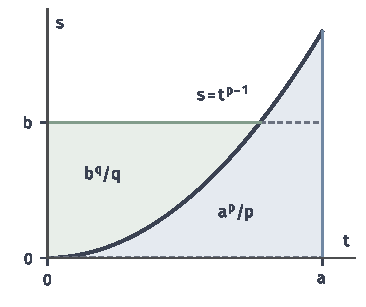
\includegraphics[width=62mm]{figures/04-spaces-measures-and-geometry/03-function-spaces/matplotlib/nspace-young-area/figure.pdf}
  \caption{Young不等式的面积解释，取$p=3$、$q=\tfrac32$、$a=1$、$b=0.6$。曲线为$s=t^2$，蓝色区域面积$a^p/p=\tfrac13$，绿色区域面积$b^q/q\approx0.310$，二者盖住虚线所示面积为$ab=0.6$的矩形。只有曲线恰好穿过矩形右上角，即$b=a^{p-1}$时，两块区域才恰好拼成矩形。}
  \label{fig:nspace-young-area}
\end{BookInlineFigure}

用图中的数字验算：$ab=0.6$，而$\tfrac13+0.310=0.643$，不等式成立且是严格的。若把$b$取成$a^{p-1}=1$，则$ab=1=\tfrac13+\tfrac23$，等号成立。

\begin{theorem}[Hölder不等式]
\label{thm:nspace-holder}
设$1<p<\infty$，$q$为其共轭指数，$f,g$是$X$上的可测函数。则
\begin{equation}
 \int_X\lvert fg\rvert\,d\mu\leq\lVert f\rVert_p\,\lVert g\rVert_q ,
 \label{eq:nspace-holder}
\end{equation}
其中右边允许取$+\infty$。特别地，$f\in L^p(\mu)$、$g\in L^q(\mu)$时$fg\in L^1(\mu)$。
\end{theorem}

\begin{proof}
若右边为$+\infty$，无需证明。若$\lVert f\rVert_p=0$，则$f=0$几乎处处，$fg=0$几乎处处，左边为零；$\lVert g\rVert_q=0$同理。下设$0<\lVert f\rVert_p,\lVert g\rVert_q<\infty$。

在Young不等式中逐点取$a=\lvert f(x)\rvert/\lVert f\rVert_p$、$b=\lvert g(x)\rvert/\lVert g\rVert_q$，得到
\[
 \frac{\lvert f(x)g(x)\rvert}{\lVert f\rVert_p\lVert g\rVert_q}\leq\frac{\lvert f(x)\rvert^p}{p\lVert f\rVert_p^p}+\frac{\lvert g(x)\rvert^q}{q\lVert g\rVert_q^q}.
\]
两边积分，右边等于$\tfrac1p+\tfrac1q=1$，再乘以$\lVert f\rVert_p\lVert g\rVert_q$即得结论。
\end{proof}

归一化的作用是把两个任意大小的函数缩放到“单位大小”，使右边两项积分后恰好凑成$1$。在$[0,1]$上取$f=x$、$g=x^2$、$p=3$、$q=\tfrac32$，此时$\lvert f\rvert^3=x^3=\lvert g\rvert^{3/2}$，两边相等：
\[
 \int_0^1x^3\,dx=\frac14,\qquad \Bigl(\frac14\Bigr)^{1/3}\Bigl(\frac14\Bigr)^{2/3}=\frac14,
\]
这与Young不等式的等号条件$a^p=b^q$相符。若取$f=1$、$g=x$、$p=q=2$，左边为$\tfrac12$，右边为$(\tfrac13)^{1/2}\approx0.577$，不等式是严格的。

\begin{theorem}[Minkowski不等式]
\label{thm:nspace-minkowski}
设$1\leq p<\infty$，$f,g\in L^p(\mu)$。则
\begin{equation}
 \lVert f+g\rVert_p\leq\lVert f\rVert_p+\lVert g\rVert_p.
 \label{eq:nspace-minkowski}
\end{equation}
因此$(L^p(\mu),\lVert\cdot\rVert_p)$是赋范空间。
\end{theorem}

\begin{proof}
$p=1$时，对逐点不等式$\lvert f+g\rvert\leq\lvert f\rvert+\lvert g\rvert$积分即可。

设$1<p<\infty$，记$I=\int\lvert f+g\rvert^p\,d\mu$。由封闭性的估计，$I<\infty$；若$I=0$，结论平凡，下设$I>0$。先把$p$次幂拆成两项：
\[
 \lvert f+g\rvert^p\leq\lvert f+g\rvert^{p-1}\lvert f\rvert+\lvert f+g\rvert^{p-1}\lvert g\rvert.
\]

由$(p-1)q=p$，$\lvert f+g\rvert^{p-1}$的$q$次积分等于$I$，所以它的$L^q$范数是$I^{1/q}$。对右边两项分别用Hölder不等式，
\[
 \int\lvert f+g\rvert^{p-1}\lvert f\rvert\,d\mu\leq I^{1/q}\lVert f\rVert_p,
\]
\[
 \int\lvert f+g\rvert^{p-1}\lvert g\rvert\,d\mu\leq I^{1/q}\lVert g\rVert_p.
\]

相加，得到
\[
 I\leq I^{1/q}\bigl(\lVert f\rVert_p+\lVert g\rVert_p\bigr).
\]
两边除以$I^{1/q}$（它有限且为正），由$1-\tfrac1q=\tfrac1p$得$I^{1/p}\leq\lVert f\rVert_p+\lVert g\rVert_p$，这就是结论。
\end{proof}

证明中的除法要求$I$有限且为正：有限性来自封闭性估计，正性单独处理。若只知道$I\leq I^{1/q}(\cdots)$而不知$I<\infty$，两边可能都是$\infty$，推不出结论。

\paragraph{完备性}
现在回答本节开头的问题：积分误差下的柯西列是否一定有极限。困难在于$L^p$范数只控制积分，不控制每一点：柯西列在单个点处可能根本不收敛。第~\ref{sec:nspace-convergence-of-sequences}节的打字机序列就是这样。

下面的证明先抽出一个相邻误差可求和的子列，借它得到几乎处处收敛的候选极限，再用Fatou引理把逐点信息转回积分。

\begin{theorem}[$L^p$的完备性]
\label{thm:nspace-lp-complete}
对任意测度空间与$1\leq p<\infty$，$L^p(\mu)$是Banach空间。
\end{theorem}

\begin{proof}
设$(f_n)$是$L^p(\mu)$中的柯西列，取定各项的可测代表。

第一步，抽取快速子列。由柯西条件，可以递归地取$n_1<n_2<\cdots$，使$m,n\geq n_k$时$\lVert f_n-f_m\rVert_p<2^{-k}$。于是
\[
 \lVert f_{n_{k+1}}-f_{n_k}\rVert_p<2^{-k},\qquad \sum_{k\geq1}\lVert f_{n_{k+1}}-f_{n_k}\rVert_p<\infty.
\]

第二步，构造控制函数。令
\[
 S_m=\lvert f_{n_1}\rvert+\sum_{k=1}^m\lvert f_{n_{k+1}}-f_{n_k}\rvert,\qquad S=\lim_{m\to\infty}S_m\in[0,\infty].
\]
由Minkowski不等式，$S_m$的范数有一个与$m$无关的上界：
\[
 \lVert S_m\rVert_p\leq\lVert f_{n_1}\rVert_p+\sum_{k\geq1}\lVert f_{n_{k+1}}-f_{n_k}\rVert_p=:C<\infty.
\]
$S_m^p$逐点单调上升到$S^p$，由单调收敛定理，
\[
 \int_XS^p\,d\mu=\lim_{m\to\infty}\int_XS_m^p\,d\mu\leq C^p.
\]
所以$S<\infty$几乎处处。

第三步，定义候选极限。在$\{S<\infty\}$上，级数$f_{n_1}+\sum_k(f_{n_{k+1}}-f_{n_k})$绝对收敛，它的第$k$个部分和就是$f_{n_{k+1}}$；令$f$为其和，在零测集$\{S=\infty\}$上令$f=0$。$f$是可测函数列的几乎处处极限，因而可测，并且$\lvert f\rvert\leq S$，所以$f\in L^p(\mu)$。

第四步，子列依范数收敛。固定$j$。在$\{S<\infty\}$上，
\[
 \lvert f-f_{n_j}\rvert^p=\lim_{m\to\infty}\lvert f_{n_m}-f_{n_j}\rvert^p.
\]
由Fatou引理，
\[
 \int_X\lvert f-f_{n_j}\rvert^p\,d\mu\leq\liminf_{m\to\infty}\int_X\lvert f_{n_m}-f_{n_j}\rvert^p\,d\mu.
\]
把差写成相邻差之和，
\[
 f_{n_m}-f_{n_j}=\sum_{k=j}^{m-1}\bigl(f_{n_{k+1}}-f_{n_k}\bigr),
\]
再用Minkowski不等式，得到
\[
 \lVert f-f_{n_j}\rVert_p\leq\sum_{k\geq j}\lVert f_{n_{k+1}}-f_{n_k}\rVert_p.
\]
右边是收敛级数的尾和，趋于零，所以$\lVert f_{n_j}-f\rVert_p\to0$。

第五步，回到整列。给定$\varepsilon>0$，取$N$使$m,n\geq N$时$\lVert f_n-f_m\rVert_p<\varepsilon$，再取$j$使$n_j\geq N$且$\lVert f_{n_j}-f\rVert_p<\varepsilon$。则$n\geq N$时
\[
 \lVert f_n-f\rVert_p\leq\lVert f_n-f_{n_j}\rVert_p+\lVert f_{n_j}-f\rVert_p<2\varepsilon.
\]
\end{proof}

五步各有职责。第一步的快速子列使控制函数$S$的范数有限；第二步由此得到$S<\infty$几乎处处，候选极限才有定义；第四步的Fatou引理把几乎处处的收敛转化为积分误差的估计；最后一步说明：柯西列只要有一个子列收敛，整列就收敛到同一极限。

图~\ref{fig:nspace-fast-subsequence}用一列具体的函数显示了第二步的控制。部分和不断加上越来越小的修正，$S_m$把所有修正的绝对值累计起来，单调上升但有界；$f_{n_k}$始终夹在$-S$和$S$之间，所以每个$S<\infty$的点处级数都绝对收敛。

\begin{BookInlineFigure}
  \centering
  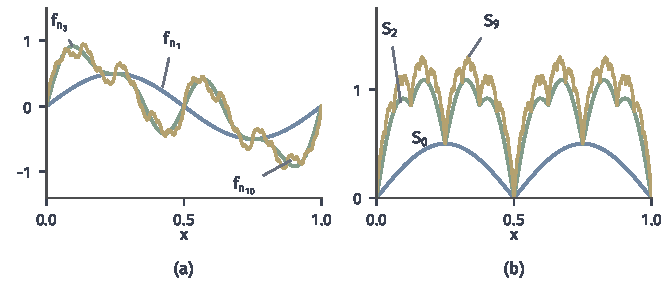
\includegraphics[width=112mm]{figures/04-spaces-measures-and-geometry/03-function-spaces/matplotlib/nspace-fast-subsequence/figure.pdf}
  \caption{完备性证明中的快速子列与控制函数。这里$f_{n_1}(x)=\tfrac12\sin(2\pi x)$，相邻差$f_{n_{k+1}}-f_{n_k}=2^{-k}\sin(2^{k+1}\pi x)$。(a)$f_{n_1},f_{n_3},f_{n_{10}}$，修正项越来越小。(b)控制函数$S_0,S_2,S_9$，随$m$单调上升且有界，每一项$\lvert f_{n_k}\rvert$都不超过它们的极限$S$。}
  \label{fig:nspace-fast-subsequence}
\end{BookInlineFigure}

\begin{theorem}[$L^p$收敛列的几乎处处收敛子列]
\label{thm:nspace-lp-ae-subsequence}
设$1\leq p<\infty$，在$L^p(\mu)$中$f_n\to f$。则存在子列$(f_{n_k})$，使$f_{n_k}\to f$几乎处处成立。
\end{theorem}

\begin{proof}
收敛列是柯西列。定理~\ref{thm:nspace-lp-complete}证明的前四步给出子列与函数$\tilde f$，使$f_{n_k}\to\tilde f$几乎处处且在$L^p$中成立。$L^p$中的极限唯一，所以$\tilde f=f$几乎处处，于是$f_{n_k}\to f$几乎处处。
\end{proof}

回到上一节的折线列$(g_n)$，把证明的步骤走一遍。在$L^1[0,1]$中，阶跃函数的等价类$\mathbf 1_{(1/2,1]}$是合法的元素。由式~\eqref{eq:nspace-ramp-distance}，取$n_k=2^k$时相邻误差为
\[
 \lVert g_{2^{k+1}}-g_{2^k}\rVert_1=\frac1{2^{k+1}}-\frac1{2^{k+2}}=2^{-k-2},
\]
对$k\geq1$求和得$\tfrac14$。

$g_n$关于$n$单调不减，所以控制函数中的绝对值可以去掉，并逐项相消：
\[
 S_m=g_2+\sum_{k=1}^m\bigl(g_{2^{k+1}}-g_{2^k}\bigr)=g_{2^{m+1}}.
\]
令$m\to\infty$，得到$S=\mathbf 1_{(1/2,1]}$，这正是候选极限。它的范数$\lVert S\rVert_1=\tfrac12$，恰好等于证明中的上界$C=\lVert g_2\rVert_1+\tfrac14=\tfrac14+\tfrac14$。

最后计算依范数的误差。折线与阶跃函数只在一个底为$\tfrac1n$、高为$1$的三角形上不同，所以
\[
 \lVert g_n-\mathbf 1_{(1/2,1]}\rVert_1=\frac1{2n}\to0.
\]
在$L^1$中折线列有了极限。阶跃函数在$\tfrac12$处取什么值无关紧要，这正是取等价类的用意。在计数测度下，定理~\ref{thm:nspace-lp-complete}说明每个$\ell^p$（$1\leq p<\infty$）都是Banach空间。
